%%% -*-LaTeX-*-

\chapter{Current and Future Work}
\label{cha:future-work}

Possible extensions of this model center on relaxing physical
assumptions made in section \ref{sec:problem-description}, and
incorporating more biological realism. An obvious next step is fitting
the stochastic model to experimental velocity distributions obtained
by Dr. Hlady's group. Other likely modifications include modeling
multiple types of receptors, 3D modeling of an ellipsoidal platelet,
and incorporating some simple intracellular platelet activation.

However, before presenting these broader modifications to the model,
there are two immediate changes I will make:
\begin{enumerate}
\item more realistic treatment of the hydrodynamic drag terms on the
  platelet,
\item and an improvement to the stochastic algorithm based on the
  modified next reaction method of David Anderson \cite{Anderson2007}
  that simulates stochastic chemical kinetics with time-dependent rate
  functions. 
\end{enumerate}

\section{Immediate modifications to the model}
\label{sec:immed-modif-model}

The two improvements discussed below are minor adjustments to the
model to tweak the drag forces experienced by the platelet (section
\ref{sec:height-depend-fluid}) and improve the numerical algorithm
used for stochastic platelet rolling (section
\ref{sec:modif-next-react}).

\subsection{Height-dependent fluid resistance}
\label{sec:height-depend-fluid}

Assumption 3 in section \ref{sec:geometry-physics} states that drag
forces are calculated assuming that the platelet is moving in an
unbounded domain. This results in a decoupled set of linear equations
relating the force $\horzTotalForce$ and torque $\totalTorque$ exerted
by the bonds on the platelet with the translational and angular
velocities of the platelet (equations \eqref{eq:force-bal} and
\eqref{eq:torque-bal}). A more realistic treatment of the drag on a
sphere near a plane wall is one where the drag force and torque is
related to $(\velocity, \rotation)$ by a $2 \times 2$ linear
system. Goldman, Cox, and Brenner \cite{Goldman1967a} give asymptotic
approximations to the coefficients of this system based on a small
separation distance $\separation$ between the sphere and the wall.

To derive the necessary equations for force and torque balance,
separate the forces and torques on the platelet into 3 generalized
force vectors: $\mathbf{F}_\tn{bond}$, $\mathbf{F}_\tn{drag}$, and
$\mathbf{F}_\tn{shear}$. These vectors respectively represent the
force and torque on the platelet arising from bonds with the surface,
drag on the sphere generated by a sphere moving through a stationary
fluid, and drag on a stationary sphere by a shear flow. Because we are
assuming Stokes flow and ignoring all other forces, these three forces
have to balance:
\begin{equation}
  \label{eq:new-force-bal}
  0 = \mathbf{F}_\tn{bond} + \mathbf{F}_\tn{drag} + \mathbf{F}_\tn{shear}.
\end{equation}

The force generated by bonds with the surface are calculated the same
way as before, and
$\mathbf{F}_\tn{bond} = (\horzTotalForce, \totalTorque)^T$. The two
drag forces $\mathbf{F}_\tn{drag}$ and $\mathbf{F}_\tn{shear}$ are
calculated using formulae derived in \cite{Goldman1967a} and
\cite{Goldman1967b} respectively.

From \cite{Goldman1967a},
\begin{equation}
  \label{eq:goldman-dforce}
  \mathbf{F}_\tn{drag} =
  \begin{pmatrix}
    6\pi\mu\radius \left(\velocity F^{t^*} + \radius\rotation F^{r^*}
    \right) \\
    8\pi\mu\radius^2 \left(\velocity T^{t^*} + \radius\rotation
      T^{r^*} \right)
  \end{pmatrix}
\end{equation}
where
\begin{align}
  F^{t^*} &= \frac{8}{15} \log\left( \frac{\separation}{\radius}
            \right) - 0.9588 \\
  F^{r^*} &= -\frac{2}{15} \log\left( \frac{\separation}{\radius}
            \right) - 0.2526 \\
  T^{t^*} &= -\frac{1}{10} \log\left( \frac{\separation}{\radius}
            \right) - 0.1895 \\
  T^{r^*} &= \frac{2}{5} \log\left( \frac{\separation}{\radius}
            \right) - 0.3817.
\end{align}

From \cite{Goldman1967b},
\begin{equation}
  \label{eq:goldman-sforce}
  \mathbf{F}_\tn{shear} =
  \begin{pmatrix}
    6\pi\mu\radius(\radius + \separation)\shear F^{s^*} \\
    4\pi\mu\radius^3 \shear T^{s^*}
  \end{pmatrix}
\end{equation}
where values of $F^{s^*}$ and $T^{s^*}$ are tabulated for different
separations $\separation$ in Table 1 of \cite{Goldman1967b}. By
extrapolation, they find that $F^{s^*} \rightarrow 1.7005$ and
$T^{s^*} \rightarrow 0.9440$ as $\separation \rightarrow 0$. These
values can be used for a crude estimate of the shear forces, or a more
accurate estimate can be calculated by interpolating the data in
\cite{Goldman1967b}.

Putting all of this together, the new force balance equations become:
\begin{align}
  \label{eq:new-force-bal}
  0 &= \horzTotalForce + 6\pi\mu\radius \left(\velocity F^{t^*} +
      \radius\rotation F^{r^*} + \appliedVel F^{s^*}
      \right) \\
  \label{eq:new-torque-bal}
  0 &= \totalTorque + 8\pi\mu\radius^2 \left(\velocity T^{t^*} +
      \radius\rotation T^{r^*} + \radius\appliedRot T^{s^*}
      \right)
\end{align}
where $\appliedVel = (\radius + \separation)\shear$ and
$\appliedRot = \shear/2$. Equations (\ref{eq:force-bal}) and
(\ref{eq:torque-bal}) are specific instances of
(\ref{eq:new-force-bal}) and (\ref{eq:new-torque-bal}) with
$F^{t^*} = T^{r^*} = -1$, $F^{r^*} = T^{t^*} = 0$, and
$F^{s^*} = T^{s^*} = 1$. The same coefficients for a separation
distance $\separation = 10 \, \tn{nm}$ are given in Table
\ref{tab:nondim-drag}.

\begin{table}
  \centering
  \begin{tabular}{ll}
    \toprule
    Coefficient & Value \\
    \midrule
    $F^{t^*}$ & -3.4149 \\
    $F^{r^*}$ & 0.3614 \\
    $F^{s^*}$ & 1.7005 \\
    $T^{t^*}$ & 0.2710 \\
    $T^{r^*}$ & -2.2238 \\
    $T^{s^*}$ & 0.9440 \\
    \bottomrule
  \end{tabular}
  \caption[Nondimensional drag coefficients]{Nondimensional factors
    for hydrodynamic shear with a separation distance $\separation =
    10 \, \tn{nm}$ from Goldman, Cox, and Brenner.}
  \label{tab:nondim-drag}
\end{table}

\subsection{Modified next reaction method for platelet rolling}
\label{sec:modif-next-react}

There are a couple of weaknesses in the naive approach described in
section \ref{sec:modif-gill-algor}. First, because the algorithm
requires two random numbers for every single time step, and in
practice the maximum time step enforced is much smaller than the
average time for a bond to form or break, the algorithm discards most
of the random numbers generated. A typical simulation requires
$\sim10^4$ time steps, even though only $\sim10$--$100$ reactions
occur in a single simulation. That is, a single simulation generates
20,000 random numbers, but discards all but 20--200 of them.

The second problem is that this method is an inefficient way to
integrate the motion of the platelet. The motion of a rolling platelet
is piecewise deterministic: that is, in between bond formation and
breaking events, the motion of the platelet is deterministic. The
method described above is really integrating the motion of the
platelet using a forward Euler method with a constant step size. This
is a poor choice, because the nondimensional friction coefficient for
the platelet motion is very small, and the ODEs governing platelet
motion are stiff. Therefore the stability condition for Forward Euler
requires a very small step size. In summary, there are two distinct
pieces of a stochastic simulation of platelet rolling: the
deterministic motion of the platelet, and the stochastic bond
formation and breaking between the platelet and surface.

To more clearly separate the integration of the deterministic
equations of motion for the platelet from random binding and unbinding
events, we can adapt the modified next reaction method
\cite{Anderson2007} to platelet rolling. The modified next reaction
method exactly simulates a stochastic chemical system with
time-varying reaction rate functions. The details of this method are
explained in Appendix \ref{cha:numerical-schemes}, but I will
summarize the main points here.

The main idea behind the modified next reaction method is to keep
track of the ``internal time'' of each reaction. The internal time is
essentially a nondimensionalization of the absolute simulation time so
that each reaction fires at a unit rate in its own internal time. At
the beginning of a simulation, exponentially distributed random
numbers are generated for each reaction which become the
\emph{internal} firing times for each reaction. As the external time
of the system is advanced, the internal clocks of the reactions
advance at different speeds based on the propensity of each particular
reaction. The internal clock of a reaction with a high propensity
advances quickly, whereas the internal clock of a reaction with a low
propensity advances more slowly. For a reaction $k$, the internal time
of that reaction is denoted as $T_k$, and it is related to the
external time $t$ by an integral of its reaction propensity
$a_k(t, X(t))$: $T_k(t) = \Int{a_k(s, X(s))}{s}{0}{t}$.

The algorithm proceeds until one of the internal clocks reaches its
firing time. Then the system is updated according to whichever
reaction fires, the new reaction rates are calculated, and a new
internal firing time is chosen for the reaction which fired. Then this
process iterates until the end time of the simulation is reached. The
modified next reaction method can be applied directly to our platelet
rolling model, with one alteration: internal timers have to
initialized and discarded throughout the simulation as bonds form and
break. As illustrated in Figure \ref{fig:internal-clocks}, each bin on
the surface of the platelet has its own internal clock, and each
existing bond has its own clock.

\begin{figure}
  \centering
  \includegraphics[width=0.5\textwidth]{internal-clocks}
  \caption[Internal clocks in the modified stochastic method for
  platelet rolling.]{Internal clocks in modified stochastic method for
    platelet rolling. Each reaction has its own internal time which
    can be converted to absolute time. Reactions with high reaction
    rates have internal clocks which advance more quickly than
    reactions with lower rates.}
  \label{fig:internal-clocks}
\end{figure}

Of course, this method for simulating stochastic bond chemistry has to
be implemented along with a solver for a set of ODEs governing the
motion of the platelet due to force balance between bonds and the
fluid. The equations which define platelet motion in the stochastic
rolling simulation are:
\begin{equation}
  \label{eq:motion-odes}
  \renewcommand*{\arraystretch}{1.5}
  \begin{pmatrix}
    F^{t^*} & \radius F^{r^*} \\
    T^{t^*}/\radius & T^{r^*}
  \end{pmatrix}
                      \begin{pmatrix}
                        \Der{\wallDist_\tn{ref}}{\dTime} \\
                        \Der{\recAngle}{\dTime}
                      \end{pmatrix}
            =
              \begin{pmatrix}
                \horzTotalForce(\wallDist_\tn{ref},
                \recAngle_\tn{ref}) / 6\pi\mu\radius + \appliedVel
                F^{s^*} \\
                \totalTorque(\wallDist_\tn{ref}, \recAngle_\tn{ref}) /
                8\pi\mu\radius^3 + \appliedRot T^{s^*}
              \end{pmatrix}
\end{equation}
where $\wallDist_\tn{ref}$ and $\recAngle_\tn{ref}$ are reference
coordinates and the coordinates giving the endpoints of bond $i$ are
defined by
$\wallDist_i(\dTime) = \wallDist_\tn{ref}(\dTime) + \wallDist_i^0$ and
$\recAngle_i(\dTime) = \recAngle_\tn{ref}(\dTime) +
\recAngle_i^0$. The system (\ref{eq:motion-odes}) can be integrated by
any standard ODE solver to find $\wallDist_\tn{ref}(\dTime)$ and
$\recAngle_\tn{ref}(\dTime)$. Once the reference coordinates are known
as a function of time, the reaction rates $a_k(t, X(t))$ are known as
functions of $\dTime$ up until the next reaction.

To my knowledge, this method has not been implemented in the context
of cell rolling before. All of the papers referenced above either use
a method that is similar to the modified Gillespie method described in
section \ref{sec:stochastic-model}, or use a fixed time step method
where multiple reactions can occur in a single time step. I expect
this method to improve the efficiency of stochastic simulations of my
model, by allowing the use of a higher-order and/or more stable method
to integrate the deterministic ODE system for platelet position, and
discarding far fewer random numbers than the Gillespie approach.

\section{Fit stochastic parameters to experimental data}
\label{sec:fit-stoch-param}

One advantage of the stochastic algorithm is that it is able to
model the full velocity distribution of a population of platelets all
interacting with an agonist-coated surface. Experimental observations
show that platelets go through a wide range of rolling velocities in
the course of an experiment, indicating that stochasticity is
important, and it also highlights a deficiency of the deterministic
model in that it can only reproduce the mean rolling velocity of
platelets.

Dr. Hlady's group has characterized platelet rolling on an
agonist-coated surface in several different ways that provide
different checks on the stochastic algorithm. The different statistics
that are calculated from platelet rolling may not be independent
of one another, but nonetheless the stochastic algorithm should be
able to capture the same behaviors. The rolling data collected are:
\begin{itemize}
\item platelet pause/dwell times (i.e. the length of time a platelet
  spends stationary or almost stationary on the surface before
  resuming rolling),
\item platelet instantaneous and time-averaged velocities, and
\item platelet step sizes (i.e. the distance a platelet travels in
  between pause events).
\end{itemize}

All of these features have analogs in the stochastic model which can
be tracked and recorded to compare with experimental data. In the
deterministic model, there are no pauses and therefore it produces
nothing that can be compared to experimental measurements of pause
times or step sizes, in addition to the limitation that it cannot
produce a distribution of platelet velocities.

What parameters can be fit to this experimental data? Many of the
parameters in this model have been estimated before in other research
on platelet rolling, both in modeling work
\cite{Fitzgibbon2014,Mody2008b,Wang2013} and in experimental papers
\cite{Litvinov2011,Litvinov2012}. However the confidence in these
parameter estimates varies depending on the parameter. For example,
the bond formation rate is difficult to estimate precisely and can
only be estimated to within several orders of magnitude. In addition,
some of these parameters with platelet priming. For example, it is
known that more adhesion receptors are recruited to the surface during
platelet activation. It is also known that integrins \ITA{IIb}\ITB{3}
and \ITA{2}\ITB{1} are activated as a result of platelet activation
\cite{Kee2015}, which may change any or all of $\onConst$,
$\offConst$, $\refForce$, $\stiffness$, or $\compliance$. By modifying
these parameters, we can crudely model platelet activation in the
model presented above.

\section{Multiple types of receptors}
\label{sec:multiple-receptors}

One fairly obvious extension of the model is to model 2 different
receptors with different parameters. For platelet agonists vWF and
collagen, there are two receptors which can bind with each of these
receptors: GP1b and \ITA{IIb}\ITB{3} for vWF, and GPIV and
\ITA{2}\ITB{1} for collagen. GP1b and GPIV are fast receptors with
relatively large binding and unbinding rates, and these receptors are
constitutively present and active on the surfaces of inactive
platelets and do not change their activity based on the platelet's
activation state.

On the other hand, the integrin receptors \ITA{IIb}\ITB{3} and
\ITA{2}\ITB{1} have smaller binding and unbinding rates, and therefore
mediate firm adhesion. In addition, while they are constitutively
expressed on the surface of inactive platelets, these receptors are
in their low-affinity conformation until the platelet is activated and
intracellular signaling pathways signal the integrins to switch to
their high-affinity conformation.

The idea to perform rolling simulations with two different receptors
with different binding kinetics is not a new one. For example, Bhatia
et. al. \cite{Bhatia2003} demonstrated how different behaviors of
leukocyte rolling can be found by varying concentrations of two
different ligands. To my knowledge, there is no similar analysis for
platelets. I would not expect qualitatively different results from
theirs which show that the two receptors act synergistically to
mediate firm adhesion, whereas either receptor acting independently
can only mediate cell rolling. However this is an important step
towards a model that includes intracellular signaling dynamics, and
simulating platelets that are able to change their chemistry in order
to transition from rolling to firm adhesion.

\section{Elliptical platelets in 3D}
\label{sec:ellipt-plat-3d}

A generalization of the model would be to model the platelet as a
rigid ellipsoid instead of as a sphere. The obvious advantage to this
approach is that it is more realistic than modeling platelets as
spheres. The disadvantage is that it greatly increases computational
cost, and may require explicit modeling of repulsive forces between
the platelet and wall to prevent platelet-wall overlap.

In the model with spherical platelets, the drag coefficients could be
calculated with analytical formulae. This is not the case for an
ellipsoid moving near a plane wall, and the drag coefficients must be
determined by solving the Stokes flow problem around the
ellipsoid. Specifically, the problem we need to solve is the
following:
\begin{align}
  \label{eq:3D-stokes-mom}
  0 &= -\nabla p(\mathbf{x}) + \mu \Delta \mathbf{u}(\mathbf{x}) \quad
      \tn{for} \quad \mathbf{x} \in W \setminus D \\
  \label{eq:3D-stokes-inc}
  0 &= \nabla \cdot \mathbf{u}.
\end{align}
Here $W = \left\{(x', y', z') \in \reals^3 \mid z' > 0\right\}$ is the
region above the plane wall, $D$ is the interior of the ellipsoid, and
$\mathcal{S} \equiv \partial D$ is the surface of the ellipsoid. Equations
(\ref{eq:3D-stokes-mom}) and (\ref{eq:3D-stokes-inc}) are solved with
no-slip boundary conditions on the wall ($\mathbf{u} = 0$ for $z'=0$)
and on the ellipsoid
($\mathbf{u} = \mathbf{V} + \mathbf{x} \times \mathbf{\Omega}$), and
with the far-field condition
$\mathbf{u}(\mathbf{x}) \rightarrow \shear z'$ as
$\|\mathbf{x}\| \rightarrow \infty$. This problem can be separated
into a problem with an ellipsoid moving through a stationary fluid and
an ellipsoid sitting stationary in a shear flow, but the solution of
those problems only differs in the boundary conditions applied on the
surface of the platelet.

\begin{figure}
  \centering
  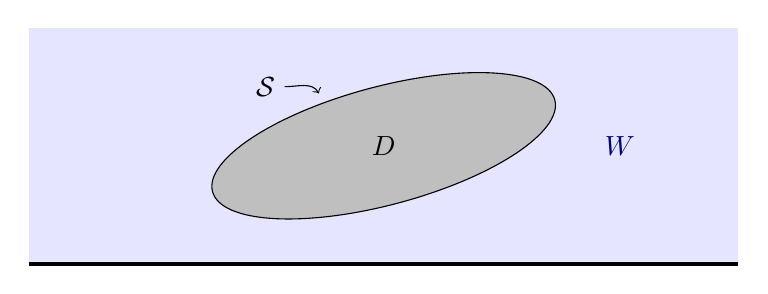
\begin{tikzpicture}[scale=1.5]
  \fill[blue!10] (-3, 0) rectangle (3, 2);
  \draw[very thick] (-3, 0) -- (3, 0);
  \draw[fill=lightgray] (0, 1) circle [x radius=1.5, y radius=.5, rotate=15];
  
  \node[blue!50!black] at (2, 1) {$W$};
  \node at (0, 1) {$D$};
  \node (label) at (-1, 1.5) {$\mathcal{S}$};
  \node (boundary) at (-.5, 1.36) {};
  \draw[->] (label) to [out=0, in=120] (boundary);
\end{tikzpicture}

  \caption[An elliptical platelet near a plane wall.]{An elliptical
    platelet near a plane wall. $W$ is the fluid region outside the
    platelet, $D$ is the region inside the platelet, and
    $\mathcal{S} \equiv \partial D$ is the surface of the platelet.}
  \label{fig:platelet}
\end{figure}

Because Stokes' equations are linear and elliptical, their solution
can be written in terms of the following boundary integral equation,
\begin{equation}
  \label{eq:bdy-int-eqn}
  u_j(\mathbf{x}) = \Int{f_i(\mathbf{x}') S_{ij}(\mathbf{x},
    \mathbf{x}')}{\mathbf{x}'}{\mathcal{S}}{}
\end{equation}
where $S_{ij}(\mathbf{x}, \mathbf{x}')$ is the wall-bounded Stokeslet
due to a point force at $\mathbf{x}'$. The benefit of using equation
(\ref{eq:bdy-int-eqn}) to find $\mathbf{u}(\mathbf{x})$ is that
discretizing (\ref{eq:bdy-int-eqn}) only requires a discretization of
a 2D surface. If we used the immersed boundary method instead, for
example, we would need to discretize the entire 3D fluid
volume. Another advantage of (\ref{eq:bdy-int-eqn}) is it solves for
the flow in the entire semi-infinite domain, something other methods
would not be able to do.

That said, there are some difficulties in using equation
(\ref{eq:bdy-int-eqn}) as well. One problem is that $S_{ij}$ is
singular on $\mathcal{S}$, and while the exact integral in
(\ref{eq:bdy-int-eqn}) is bounded, numerically evaluating an
approximate integral of a singular integrand can be
problematic. Another issue is that (\ref{eq:bdy-int-eqn}) is a
Fredholm integral equation of the 1st kind, which are often
ill-conditioned.

Regularized Stokeslets \cite{Cortez2001} are one way to deal with the
problem of a singular kernel. The main idea here is to assume forces
are distributed over a small area, instead of being concentrated at a
point. In particular, the Stokeslet $S_{ij}$ is defined so that
\begin{equation}
  \label{eq:flow-pt-force}
  u_i(\mathbf{x}) = \frac{1}{8 \pi \mu}
  S_{ij}(\mathbf{x}, \mathbf{x}') f_j
\end{equation}
solves Stokes' equations (equations (\ref{eq:stokes-momentum}) \&
(\ref{eq:stokes-mass})) for a point force of strength $\mathbf{f}$:
\begin{equation}
  \mathbf{F}(\mathbf{x}) = \mathbf{f} \delta(\mathbf{x} - \mathbf{x}').
\end{equation}
Similarly, the regularized Stokeslet $S_{ij}^\epsilon$ is defined so
that
\begin{equation}
  \label{eq:flow-blob-force}
  u_i^\epsilon(\mathbf{x}) = \frac{1}{8 \pi \mu} S_{ij}^\epsilon(\mathbf{x},
  \mathbf{x}') f_j
\end{equation}
solves Stokes' equations for a force of strength $\mathbf{f}$ that is
distributed over a small area:
\begin{equation}
  \mathbf{F}^\epsilon(\mathbf{x}) = \mathbf{f}
  \phi^\epsilon(\mathbf{x} - \mathbf{x}').  
\end{equation}
Here $\phi^\epsilon(\mathbf{x})$ is a regularized $\delta$-function,
and so has the properties $\phi^\epsilon \rightarrow \delta$ as
$\epsilon \rightarrow 0$, $\int \phi^\epsilon d\mathbf{x} = 1$, and
$\phi^\epsilon$ is radially symmetric. Then in equation
(\ref{eq:bdy-int-eqn}), $S_{ij}$ is replaced by $S_{ij}^\epsilon$.

There is some subtlety in choosing the regularization parameter
$\epsilon$. It should depend on the discretization of the surface
$\mathcal{S}$, and in \cite{Ainley2008} they choose $\epsilon \sim
h^{0.9}$ where $h$ is the diameter of their mesh. Because we are
interested in the motion of an object near a wall, the gap distance to
the wall also affects the choice of regularization parameter. In the
same paper \cite{Ainley2008}, they found that errors grow more quickly
as the mesh size $h$ increases for small gap distances than for larger
gap distances. There is no theoretical rule that optimizes the
regularization parameter $\epsilon$ for a given mesh width $h$ or
distance to the plane wall, so a good $\epsilon$ has to be found
through some trial and error.

%% Is there more to add on regularized Stokeslets?

\section{Randomly-stimulated activation dynamics}
\label{sec:intr-sign}

Ultimately, a model that attempts to describe both platelet rolling
\emph{and} activation must include some intracellular signaling. As
described in section \ref{sec:overview-clotting}, platelet activation
is a complex process involving dozens of chemical intermediates which
mediate a diverse suite of responses.

There has been a large amount of modeling work describing different
pathways within the platelet activation network, most of which include
\Ca dynamics as a central point of signal integration. A research
group at Moscow State University have published a set of models
describing intracellular platelet activation as a response to thrombin
stimulation
\cite{Shakhidzhanov2015,Sveshnikova2015,Balabin2016,Sveshnikova2016}. Other
models attempt to describe intracellular \Ca dynamics within a resting
platelet \cite{Purvis2008,Dolan2014}. Instead of modeling the
activation responses downstream of the intracellular \Ca response, all
of these models prescribe cytosolic \Ca concentration as an output and
fit parameters to experimental data of platelet cytosol \Ca
concentrations. One model that includes pathways downstream of
elevated cytosolic \Ca (specifically \ITA{IIb}\ITB{3} activation and
dense granule release) is the model of Lenoci
et. al. \cite{Lenoci2011}. They were able to accurately predict a
number of platelet responses (cytosol \Ca level, $\tn{PIP}_2$
concentration, ATP concentration, and activation of \ITA{IIb}\ITB{3})
after stimulation of PAR1, a platelet receptor for thrombin.

All of these models are developed with activation by a soluble agonist
in mind. In particular, the activation signal received is assumed to
be both temporally and spatially constant. However in the case of
platelet rolling, the platelet transiently contacts the surface and
the activation signal is transmitted through GP1b and GPVI receptors
which are randomly bound to the surface. Therefore in order to model
platelet activation by rolling on an immobilized surface, a model of
intracellular signaling must be connected with a model of rolling such
that bonds between the platelet and surface trigger the signaling
model based on the number of contacts with the surface and their
duration. Thus the signaling model could be an ODE model of chemical
kinetics with stochastic forcing from the rolling model.

\section{Summary}
\label{sec:summary-future}

Our immediate plans are to add a bit more realism to the rolling model
using the near-wall drag coefficients of a sphere from Goldman, Cox,
and Brenner \cite{Goldman1967a,Goldman1967b}, and improve the
efficiency of the stochastic simulation algorithm by implementing the
modified next reaction method of David Anderson
\cite{Anderson2007}. Also, using the velocity traces of individual
platelets in the stochastic algorithm we can find step sizes (the
distance traveled in between pause events) and dwell times (the length
of time a platelet remains stationary on the surface) to compare
simulations to experimental results. Finally, longer term goals
include the addition of multiple types of receptors to the rolling
model, the extension of the model to a 3D elliptical geometry, and
simple modeling of the intracellular platelet activation process.

% is there anything to break symmetry in the dimension perpendicular
% to flow and parallel to the wall?
% Other thought, what if we keep d the same? Obviously the center of
% mass will change in this simulation
% I don't need to include a signaling model with the ellipsoidal
% geometry model, I could just use this model with fixed chemistry...

% Local Variables:
% TeX-master: "oral-document.ltx"
% End:
